% !TEX root = ../../ThesisGchatzi.tex

\subsection{Experimental Evaluation}
\label{subsec:local_sim_search_exp}

\graphicspath{{Papers/SSTD2019/}{Papers/SIGSpatial2019/}}

Next, we report results from a comprehensive evaluation of our methods against real-world datasets.

\subsubsection{Experimental Setup}
\label{subsec:evaluation_setup_search}

\paragraph {Datasets.} We use the real-world datasets also used for experimental evaluation in Section~\ref{sec:exp_btsr}, containing diverse types of geolocated time series as detailed in Table~\ref{tab:datasets}. To test scalability, we generated a synthetic, augmented version of the Flickr dataset by slightly moving each location in a random manner and altering each time series value by a random number between $1$ and $10$. We produced three additional synthetic datasets each containing $\times 2$, $\times 3$, $\times 4$ the number of time series from the original dataset. 

\begin{table}[t]
    \centering
    \caption{Datasets and parameters used in the experiments.}
    \begin{small}
    \centering
    \begin{tabular}{lccc|cccc}
    \hline
    \multirow{2}{*}{Dataset} & Area & Number of & Length of & \multicolumn{4}{c}{Default query parameters} \\
     & (km$^2$) & locations & timeseries & $\rho$ & $\epsilon$ & $\delta$ & $k$ \\
    \hline
    Flickr & Earth & 414,967 & 96 & 30\% & 7.5\% & 20 & 30\\
    Crime & 392,000 & 362,215 & 76 & 30\% & 7.5\% & 25 & 30 \\
    Taxi & 2,500 & 417,960 & 168 & 30\% & 10\% & 20 & 30 \\
    \hline
    \end{tabular}
    \end{small}
    \label{tab:datasets}
\end{table}

\paragraph{Index and Query Parameters.} To evaluate the performance benefits observed in the experiments only based on pruning, we tuned the index parameters to fixed values. The minimum ($m$) and maximum ($M$) number of entries stored in each node are set to $40$ and $100$, respectively. For both \btsr and \sbtsr, the number of MBTS is set to 10 and for \sbtsr, the number of segments $s$ is also set to 10. The query parameters involve the spatial distance and local similarity thresholds, i.e., $\rho$, $\epsilon$, $\delta$ and $k$. The values of these parameters are set differently for each dataset, based on their characteristics; default values are shown in Table \ref{tab:datasets}. The value of $\rho$ is set relatively, by setting the covered area as a percentage of the total area. Similarly, $\epsilon$ is set as a percentage of the maximum difference between the observed values.

\paragraph{Evaluation Setting.} Each experiment is performed using a randomly selected workload of 100 queries for each dataset and we report the average response time. All indices are held in memory, while the leafs contain pointers to files with geolocated time series stored on disk. All methods were developed in Java. Tests were executed on a server with 4 CPUs, each containing 8 cores clocked at 2.13GHz, and 256 GB RAM running Debian Linux.

\subsubsection{Query Performance}
\label{subsec:query_perf}

We compare the average per query execution time for all three queries using sweep line and checkpoint methods on \btsr and the checkpoint method on \sbtsr.

\begin{figure}[!tb]
\centering
\subfloat{\fbox{
\includegraphics[width=0.375\textwidth]{Figures/legend.png}}}
\\
\subfloat[Crime]{\includegraphics[trim=0.5cm 0.5cm 0.5cm 0.5cm, clip, width=0.375\textwidth]{Figures/Plots/Crime/varying_epsSP.eps}\label{subfig:var_epsSP_crime}} \quad
\subfloat[Crime]{\includegraphics[trim=0.5cm 0.5cm 0.5cm 0.5cm, clip, width=0.375\textwidth]{Figures/Plots/Crime/varying_epsTS.eps}\label{subfig:var_epsTS_crime}} \\
\subfloat[Flickr]{\includegraphics[trim=0.5cm 0.5cm 0.5cm 0.5cm, clip, width=0.375\textwidth]{Figures/Plots/Flickr/varying_epsSP.eps}\label{subfig:var_epsSP_flickr}} \quad
\subfloat[Flickr]{\includegraphics[trim=0.5cm 0.5cm 0.5cm 0.5cm, clip, width=0.375\textwidth]{Figures/Plots/Flickr/varying_epsTS.eps}\label{subfig:var_epsTS_flickr}} \\
\subfloat[Taxi]{\includegraphics[trim=0.5cm 0.5cm 0.5cm 0.5cm, clip, width=0.375\textwidth]{Figures/Plots/Taxi/varying_epsSP.eps}\label{subfig:var_epsSP_taxi}} \quad
\subfloat[Taxi]{\includegraphics[trim=0.5cm 0.5cm 0.5cm 0.5cm, clip, width=0.375\textwidth]{Figures/Plots/Taxi/varying_epsTS.eps}\label{subfig:var_epsTS_taxi}}
\caption{Query $Q_{rr}(T_q, \rho, \epsilon, \delta)$ for varying $\rho$ and $\epsilon$.}
\label{fig:query1a}
\end{figure}

\paragraph{$Q_{rr}(T_q, \rho, \epsilon, \delta)$.} Figure \ref{fig:query1a} illustrates the query performance for varying thresholds $\rho$ and $\epsilon$ and the first column of Figure \ref{fig:exp1_sim} for varying $\delta$, on all three datasets. It is apparent that the \sbtsr with the checkpoint approach outperforms the rest in all cases. Its superior pruning power is attributed to the segmentation, which yields tighter bounds within the nodes and consequently less disk accesses. The sweep line and checkpoint methods over \btsr perform similarly in all cases. Both methods access the same nodes, but the checkpoint approach needs to examine significantly less values across time to determine local similarities. However, since all local similarity calculations take place in-memory, computation cost does not make a big difference, compared to the less node accesses required with the \sbtsr. 

More specifically, for the {\em crime} dataset, relaxing $\rho$ (Figure \ref{subfig:var_epsSP_crime}) has a negative impact on all three methods as more nodes have to be accessed and pruning depends mostly on the $\epsilon$ value. \sbtsr increasingly outperforms the rest as $\rho$ increases, due to its more aggressive pruning on local similarity. For the case of increasing $\epsilon$ (Figure \ref{subfig:var_epsTS_crime}), the result is the opposite, as this way the parameter is relaxed and more nodes get accessed. For very large $\epsilon$ values, pruning is solely based on spatial distance and all approaches perform similarly. Finally, increasing $\delta$ (Figure \ref{subfig:var_delta_crime}) also increases the difference in performance among the three approaches, while it also reduces the average query response time. This is due to large numbers of subsequences qualifying for small $\delta$ values, resulting in more node accesses. As $\delta$ increases, pruning is more rapidly improved in the case of \sbtsr due to its tighter bounds.

\begin{figure}[!tb]
\centering
\subfloat{\fbox{
\includegraphics[width=0.375\textwidth]{Figures/legend.png}}}
\\
\subfloat[Crime ($Q_{rr}$)]{\includegraphics[trim=0.5cm 0.5cm 0.5cm 0.5cm, clip, width=0.375\textwidth]{Figures/Plots/Crime/varying_delta.eps}\label{subfig:var_delta_crime}} \quad
\subfloat[Crime ($Q_{kr}$)]{\includegraphics[trim=0.5cm 0.5cm 0.5cm 0.5cm, clip, width=0.375\textwidth]{Figures/Plots/Crime/varying_k_query2.eps}\label{subfig:var_k_crime}} \\
\subfloat[Taxi ($Q_{rr}$)]{\includegraphics[trim=0.5cm 0.5cm 0.5cm 0.5cm, clip, width=0.375\textwidth]{Figures/Plots/Taxi/varying_delta.eps}\label{subfig:var_delta_taxi}} \quad
\subfloat[Taxi ($Q_{kr}$)]{\includegraphics[trim=0.5cm 0.5cm 0.5cm 0.5cm, clip, width=0.375\textwidth]{Figures/Plots/Taxi/varying_k_query2.eps}\label{subfig:var_k_taxi}} \\
\subfloat[Flickr ($Q_{rr}$)]{\includegraphics[trim=0.5cm 0.5cm 0.5cm 0.5cm, clip, width=0.375\textwidth]{Figures/Plots/Flickr/varying_delta.eps}\label{subfig:var_delta_flickr}} \quad
\subfloat[Flickr ($Q_{kr}$)]{\includegraphics[trim=0.5cm 0.5cm 0.5cm 0.5cm, clip, width=0.375\textwidth]{Figures/Plots/Flickr/varying_k_query2.eps}\label{subfig:var_k_flickr}}
\caption{Per column: $Q_{rr}(T_q, \rho, \epsilon, \delta)$ for varying $\delta$ -- $Q_{kr}(T_q, k, \epsilon, \delta)$ for varying $k$.}
\label{fig:exp1_sim}
\end{figure}

The results are similar but with larger differences for the {\em Flickr} dataset (Figures \ref{subfig:var_epsSP_flickr}, \ref{subfig:var_epsTS_flickr} and \ref{subfig:var_delta_flickr}). Intuitively, the less periodicity in a dataset, the more the benefit from segmentation; if the time series in the dataset exhibit periodicity, the bounds that will occur from applying $k$-means clustering on the whole sequences will be relatively tighter than otherwise. The Flickr dataset, due to its nature, is more random than the crime dataset, which justifies the larger differences. This explanation is also supported by the results for the {\em taxi} dataset, illustrated in Figures \ref{subfig:var_epsSP_crime}, \ref{subfig:var_epsTS_crime} and \ref{subfig:var_delta_crime}. Despite a similar behavior in varying all thresholds, the differences in average query response time among the different approaches are smaller than in the crime and Flickr datasets, due to the high daily periodicity of taxi drop-offs.

Another observation is that the execution cost for queries against the Taxi dataset is lower than that against Flickr. Although these two datasets have a similar number of locations, their spatial distribution and extent differ substantially (Taxi data spans New York city, while Flickr data spans the entire planet), which may significantly affect pruning during search. To verify this, we ran a test with a random $Q_{rr}$ query, $\rho=30\%$ and the default parameters, and we measured the number of pruned nodes. For the query against the Taxi dataset, $3017$ nodes were pruned in the tree as opposed to only $360$ nodes in the tree built for the Flickr data. Since spatial filtering is much faster with our approach, this explains the difference in execution cost against these two datasets.

\paragraph{$Q_{kr}(T_q, k, \epsilon, \delta)$.} Figures \ref{subfig:var_k_crime}, \ref{subfig:var_k_flickr} and \ref{subfig:var_k_taxi} depict the results for the $Q_{kr}(T_q, k, \epsilon, \delta)$ query for the three datasets. As $k$ increases, more nodes have to be traversed in order to fetch the additional results, and the execution time increases for all methods. Nevertheless, \sbtsr still clearly outperforms the other two algorithms.

\paragraph{$Q_{rk}(T_q, k, \rho)$.} Figures \ref{subfig:var_ks_crime}, \ref{subfig:var_ks_flickr} and \ref{subfig:var_ks_taxi} depict the results for the $Q_{rk}(T_q, k, \rho)$ query. In this case, the performance deterioration as $k$ increases is less abrupt, especially for the crime dataset, as usually the top-$k$ results are spatially closely located and are retrieved quickly. Again, the largest and smallest differences are spotted on the Flickr and taxi datasets, respectively.

\begin{figure}[!b]
\centering
\subfloat{\fbox{
\includegraphics[width=0.375\textwidth]{Figures/legend.png}}}
\\
\subfloat[Flickr ($Q_{rk}$)]{\includegraphics[trim=0.5cm 0.5cm 0.5cm 0.5cm, clip, width=0.375\textwidth]{Figures/Plots/Flickr/varying_k_query3.eps}\label{subfig:var_ks_flickr}} \quad
\subfloat[$Q_{rr}$]{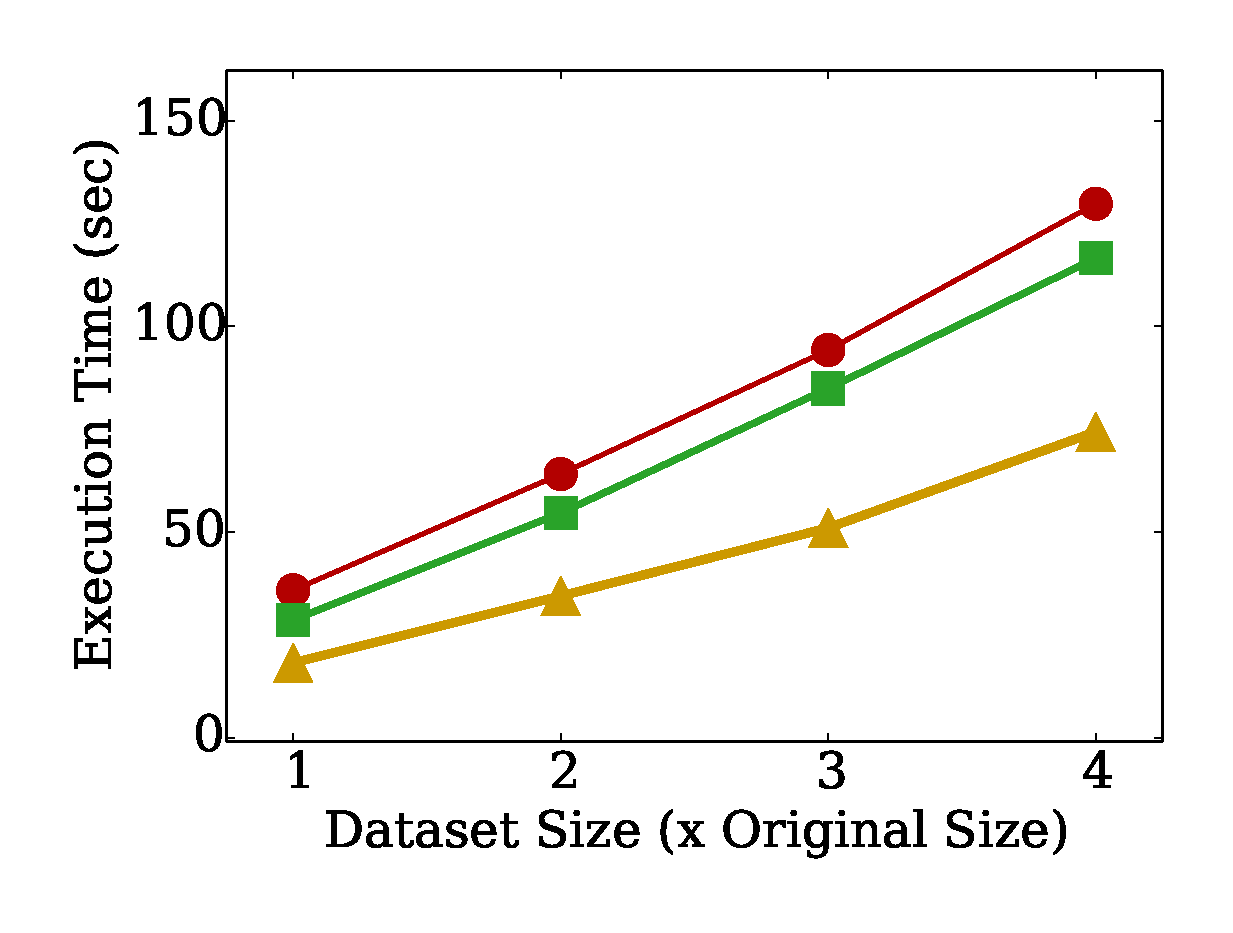
\includegraphics[trim=0.5cm 0.5cm 0.5cm 0.5cm, clip, width=0.375\textwidth]{Figures/Plots/Scalability/varyingDatasetSize_1.eps}\label{subfig:scalability1}} \\
\subfloat[Taxi ($Q_{rk}$)]{\includegraphics[trim=0.5cm 0.5cm 0.5cm 0.5cm, clip, width=0.375\textwidth]{Figures/Plots/Taxi/varying_k_query3.eps}\label{subfig:var_ks_taxi}} \quad
\subfloat[$Q_{kr}$]{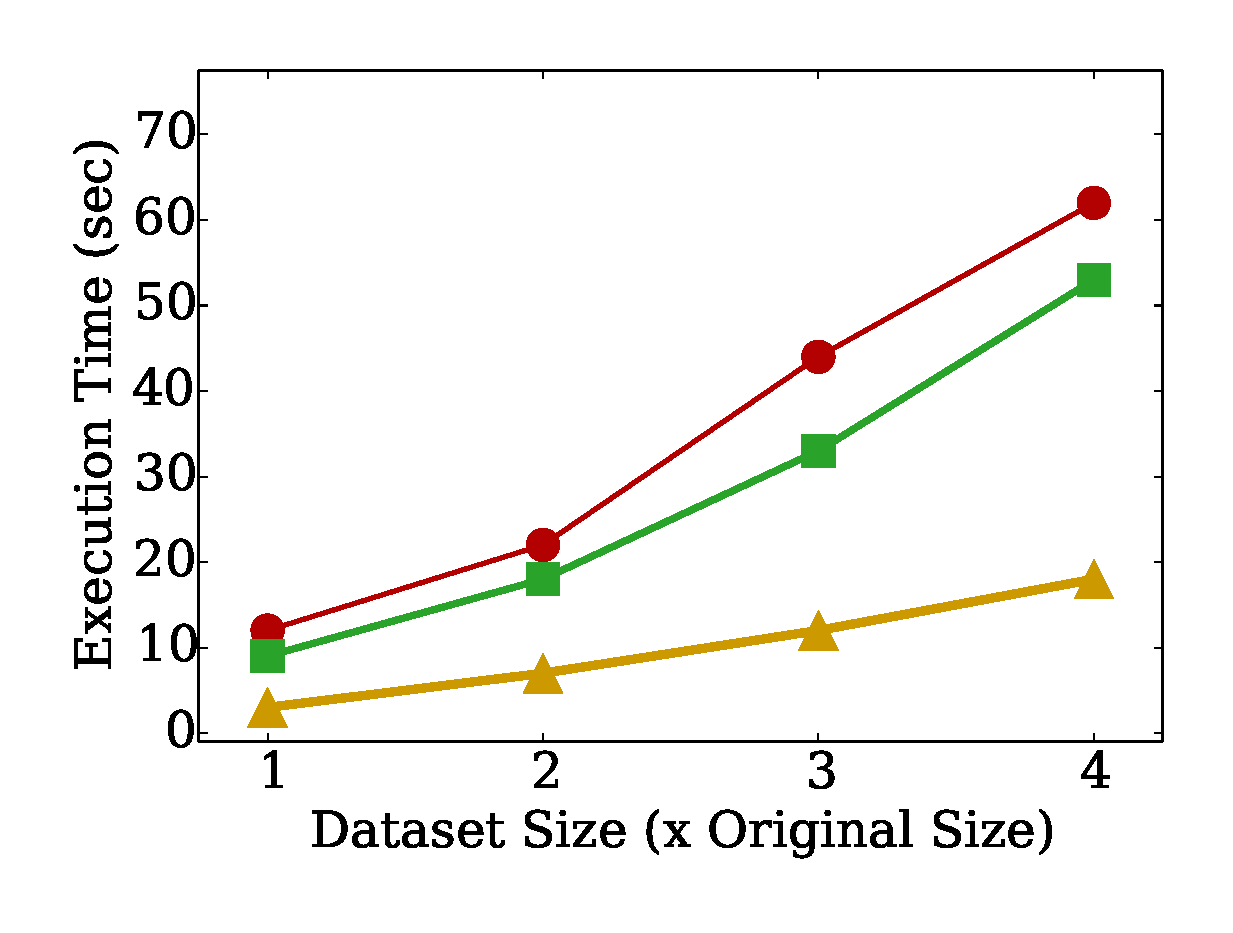
\includegraphics[trim=0.5cm 0.5cm 0.5cm 0.5cm, clip, width=0.375\textwidth]{Figures/Plots/Scalability/varyingDatasetSize_2.eps}\label{subfig:scalability2}} \\
\subfloat[Crime ($Q_{rk}$)]{\includegraphics[trim=0.5cm 0.5cm 0.5cm 0.5cm, clip, width=0.375\textwidth]{Figures/Plots/Crime/varying_k_query3.eps}\label{subfig:var_ks_crime}} \quad
\subfloat[$Q_{rk}$]{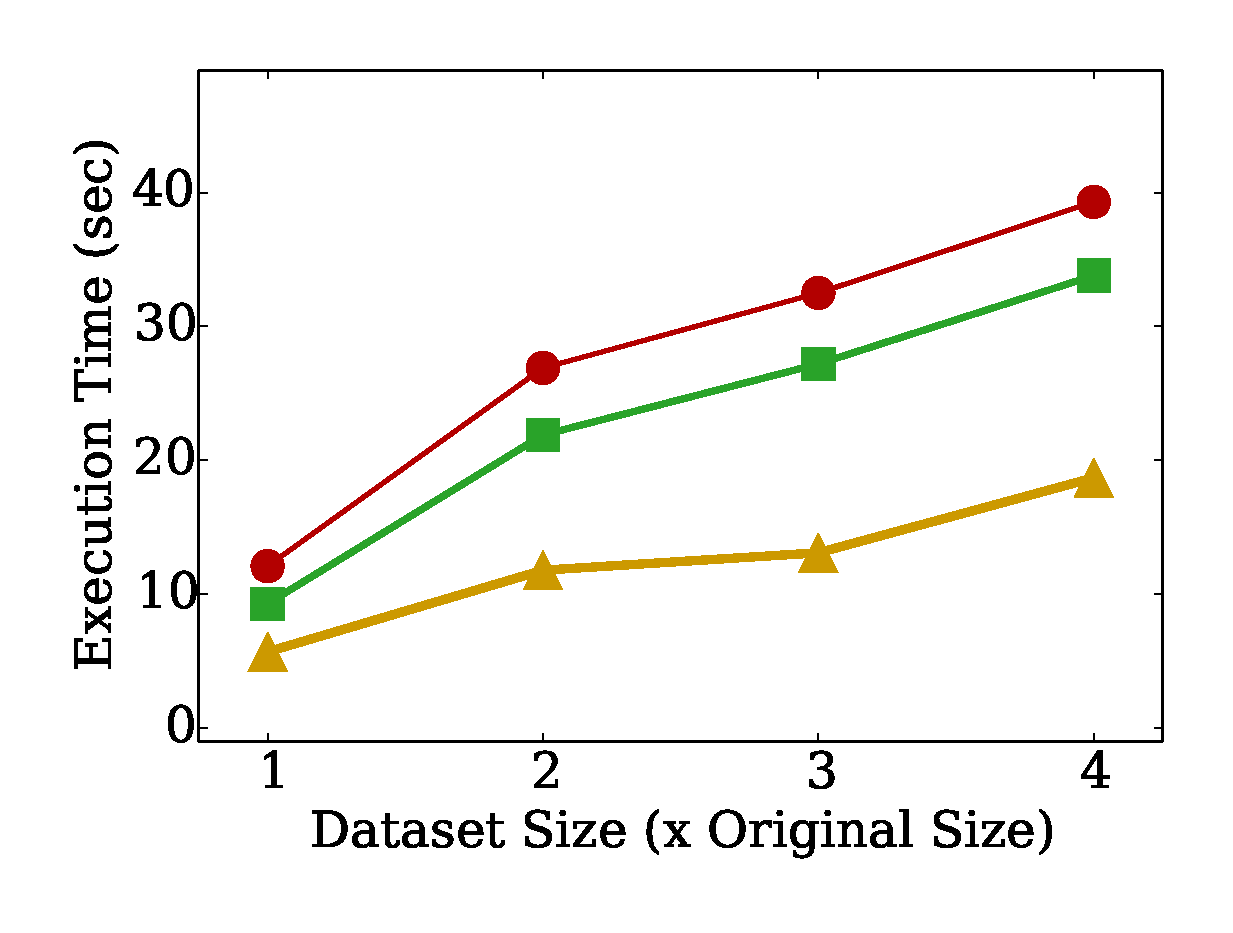
\includegraphics[trim=0.5cm 0.5cm 0.5cm 0.5cm, clip, width=0.375\textwidth]{Figures/Plots/Scalability/varyingDatasetSize_3.eps}\label{subfig:scalability3}}
\caption{Per column: $Q_{rk}(T_q, k, \rho)$ for varying $k$ -- Scalability.}
\label{fig:exp2_sim}
\end{figure}

\subsubsection{Scalability}
\label{subsec:scalability}
We performed a scalability evaluation for all three queries using the Flickr-based synthetic datasets, again measuring the average query response time for the same query workload. The results for increasing dataset size (up to four times) are depicted in Figure \ref{fig:exp2_sim}. In all cases, the \sbtsr-based approach scales better, especially in the top-$k$ queries (Figures \ref{subfig:scalability2} and \ref{subfig:scalability3}), where the larger difference observed in Figures \ref{subfig:var_k_flickr} and \ref{subfig:var_ks_flickr} is further augmented.
\\